\documentclass[fr,license=none]{../../../eplnotes}
\usepackage{float}
\usepackage[version=3]{mhchem}
\usepackage{pgfplots}
\usepackage{wrapfig}
\usepackage{siunitx}

\hypertitle{Chimie}{2}{FSAB}{1301}
{Adrien Couplet}
{Sophie Demoustier, Alain Jonas et Bernard Nysten}

\part{Atomistique}

\section{Les atomes}
\subsection{Le modèle nucléaire de l'atome}
Les premières expériences concernant la structure interne de l'atome commencèrent en 1897. Le physicien \textbf{J.J. Thomson} a découvert l'électron en étudiant les tubes cathodiques. Il découvrit qu'un tube cathodique, soumis à une différence de potentiel, crée un rayon de charges négatives venant des atomes constituant la cathode. Il en concluat que les charges négatives, qu'il appela électrons, étaient un constituant des atomes. Il détermina ensuite le rapport charge sur masse d'un électron:
$$\frac{q_e}{m_e} = \SI{-1.759e11}{\coulomb\per\kilo\gram}$$

Les valeurs de $q_e$ et $m_e$ furent découvertes plus tard en 1908 par \textbf{R. Millikan}. À l'aide de son appareil, il observa le comportement de gouttelettes d'huile chargées à travers un champ électrique. Cela lui permit de trouver la charge de l'électron, ainsi que sa masse: $$q_e = -e = \SI{-1.602e-19}{\coulomb}\qquad m_e = \SI{9.109e-31}{\kilo\gram}$$

\textbf{Rutherford} continua les recherches en envoyant des rayons alpha sur une fine feuille d'or. Il observa que certaines particules alpha étaient transmises tandis que d'autres étaient rétrodiffusées. Il suggèra alors le modèle nucléaire de l'atome. Il en conclu que l'atome était constitué d'un noyau positif entourée par un nuage d'électrons. Il émit aussi l'hypothèse de l'existence des neutrons. 
\begin{table}[H]
  \centering
  \begin{tabular}{|c|c|c|c|}\hline
    &\textbf{Masse}&\multicolumn{2}{|c|}{\textbf{Charge}}\\\hline
    &\si{\kilo\gram}&\si{\coulomb}&e\\\hline
    Proton &\num{1.673e-27}&\num{1.602e-19}&+1\\\hline
    Neutron&\num{1.675e-27}&0&0\\\hline
    Électron&\num{9.109e-31}&\num{-1.602e-19}&-1\\\hline
  \end{tabular}
  \caption{Constituants de l'atome}
  \label{tab:1}
\end{table}
Le nombre de protons dans le noyau est différent pour chaque élément. On l'appelle \textbf{nombre atomique $Z$}. Le nombre de protons et de neutrons dans le noyau est appelé le \textbf{nombre de masse $A$}. Un atome dont le nombre de neutrons est différent est appelé un isotope. On utilise la notation suivante: $$\ce{^A_ZX}$$
\subsection{Tableau de Mendeleïev}
En 1872 \textbf{D. Mendeleïev} décida de classifier les élements en fonction de leur masse atomiques et de leur affinité vis-à-vis de l'oxygène et/ou de l'hydrogène. Le tableau ne fut compléter que très récemment avec la découverte du 118$^e$ élements. On distingue dans ce tableau plusieurs groupements: les métaux alcalins, les alcalino-terreux, les métaux de transition, les métaux ``pauvres'', les métalloïdes, les non-métaux, les halogènes et les gaz nobles.
\section{Le rayonnement électromagnétique et les spectres atomiques}
La lumière visible, les ondes radio, les micro-ondes et les rayons X sont tous des types de rayonnement électromagnétique constitué d'un champ électrique oscillant et d'un champ magnétique oscillant. Toutes ces formes de rayonnement transportent de l'énergie à travers l'espace. Un rayonnement électromagnétique a plusieurs caractéristiques:
\begin{itemize}
  \item La longueur d'onde $\lambda$ est la distance entre deux pics.
  \item Le nombre de cycles par seconde est la fréquence $\nu = \frac{1}{T}$
  \item Dans le vide, un rayonnement électromagnétique se déplace à la vitesse de la lumière: $c_0=\SI{2.998e8}{\meter\per\second}$
  \item Il existe une relation entre la fréquence et la longueur d'onde: $c=\lambda\cdot\nu$
\end{itemize}
\begin{figure}[H]
  \centering
  \begin{subfigure}[b]{0.48\textwidth}\centering  
    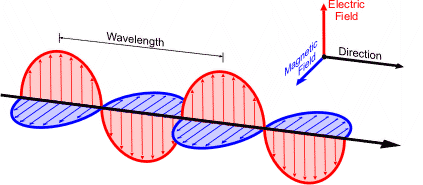
\includegraphics[width=1\textwidth]{Pictures/emwave} 
    \caption{Rayon électromagnétique}
  \end{subfigure}
  \begin{subfigure}[b]{0.48\textwidth}\centering
    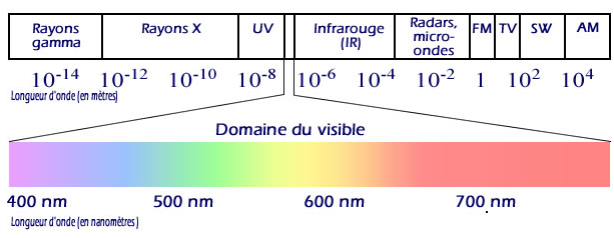
\includegraphics[width=1\textwidth]{Pictures/spectre}
    \caption{Spectre électromagnétique}
  \end{subfigure}
\end{figure}
\subsection{Diffraction des ondes électromagnétique}
La diffraction est le comportement des ondes lorsqu'elles rencontrent un obstacle ou une ouverture. La diffraction s'observe avec la lumière, mais également avec le son, les vagues, les neutrons,\dots 
\begin{figure}[H]
  \centering
  \begin{subfigure}[b]{0.48\textwidth}\centering  
    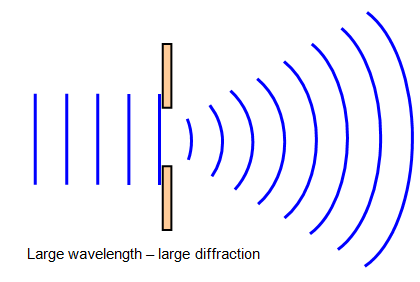
\includegraphics[width=1\textwidth]{Pictures/diffraction} 
    \caption{Diffraction optique}
  \end{subfigure}
  \begin{subfigure}[b]{0.48\textwidth}\centering
    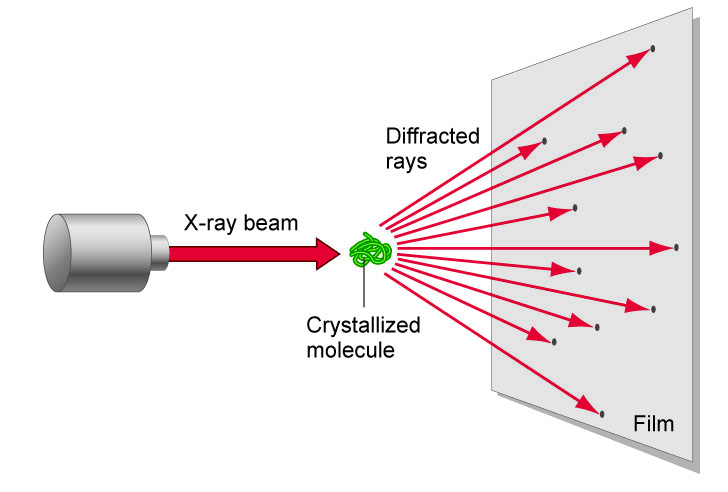
\includegraphics[width=1\textwidth]{Pictures/xray}
    \caption{Diffraction des rayons X}
  \end{subfigure}
\end{figure}
La diffraction des rayons X permet de déterminer la position des atomes d'un cristal ainsi que leurs liaisons chimique, \dots Cette méthode nécessite un faisceau de rayons X qui rencontre le cristal provoquant la dispersion du faisceau lumineux dans des directions spécifiques. Par la mesure des angles et de l'intensité des rayons, il est possible d'obtenir les informations concernant les atomes composant le cristal.
\subsection{Les différents spectres}
\begin{description}
  \item[Spectre continu]: Lorsque l'on décompose la lumière blanche à l'aide d'un prisme on observe un évantail de oculeurs. On dit que le lumière blanche possède un spectre continu, car on passe d'une couleur à une autre sans interruption.
  \item[Spectre discontinu]: Un gaz, à basse pression et à température élevée, émet une lumière constituée d'un nombre restreint de radiations : on obtient un spectre de raies d'émission ou spectre discontinu. 
  \item[Spectre d'absorption]: Lorsqu'un gaz à basse pression et à basse température est traversé par de la lumière blanche, le spectre de la lumière transmise est constitué de raies noires se détachant sur le fond coloré du spectre de la lumière blanche : c'est un spectre de raies d'absorption. La propriété importante de ce spectre de raies d'absorption est que ses raies se produisent au même endroit que les raies d'émission. 
\end{description}
\subsection{Spectre de l'hydrogène}
Lorsqu'on fait passer un courant électrique à travers de l'hydrogène gazeux sous basse pression, l'hydrogène émet de la lumière. Le courant brise les molécules de $\ce{H_2}$ et porte les atomes d'hydrogène libre à des niveaux d'énergies supérieurs. Ces atomes excités perdent rapidement leur excès d'énergie en émettant un rayonnement électromagnétique; ils se recombinent ensuite pour donner à nouveau des molécules $\ce{H_2}$. En faisant passer la lumière émise par les atomes d'hydrogène excités, on trouve que le rayonnement n'existe qu'à certaines longueurs d'onde, appelées raies spectrales. \newline
La relation entre les raies spectrales est écrite sous la forme $$\frac{1}{\lambda} = R_{\infty}\left(\frac{1}{n_1^2}-\frac{1}{n_2^2}\right)\qquad\text{avec } R_{\infty}=\SI{1.097e7}{\per\meter}$$
La constante $R_{\infty}$ est appelée la constante ``infinie'' de Rydberg.
Plusieurs séries de nombres ont été trouvées afin de déterminer la longueur d'onde des raies spectrales:
\begin{align*}
  \text{Série de Balmer (visible)}&\qquad n_1=2 ,& n_2=3,4,5,\dots\\
  \text{Série de Lyman (UV)}&\qquad n_1=1,& n_2=2,3,4,\dots\\
  \text{Série de Paschen (IR)}&\qquad n_1=3,& n_2=4,5,6,\dots
\end{align*}
\section{La théorie quantique}
\subsection{Rayonnement du ``corps noir''}
\begin{wrapfigure}{r}{0.5\textwidth}
  \begin{center}
    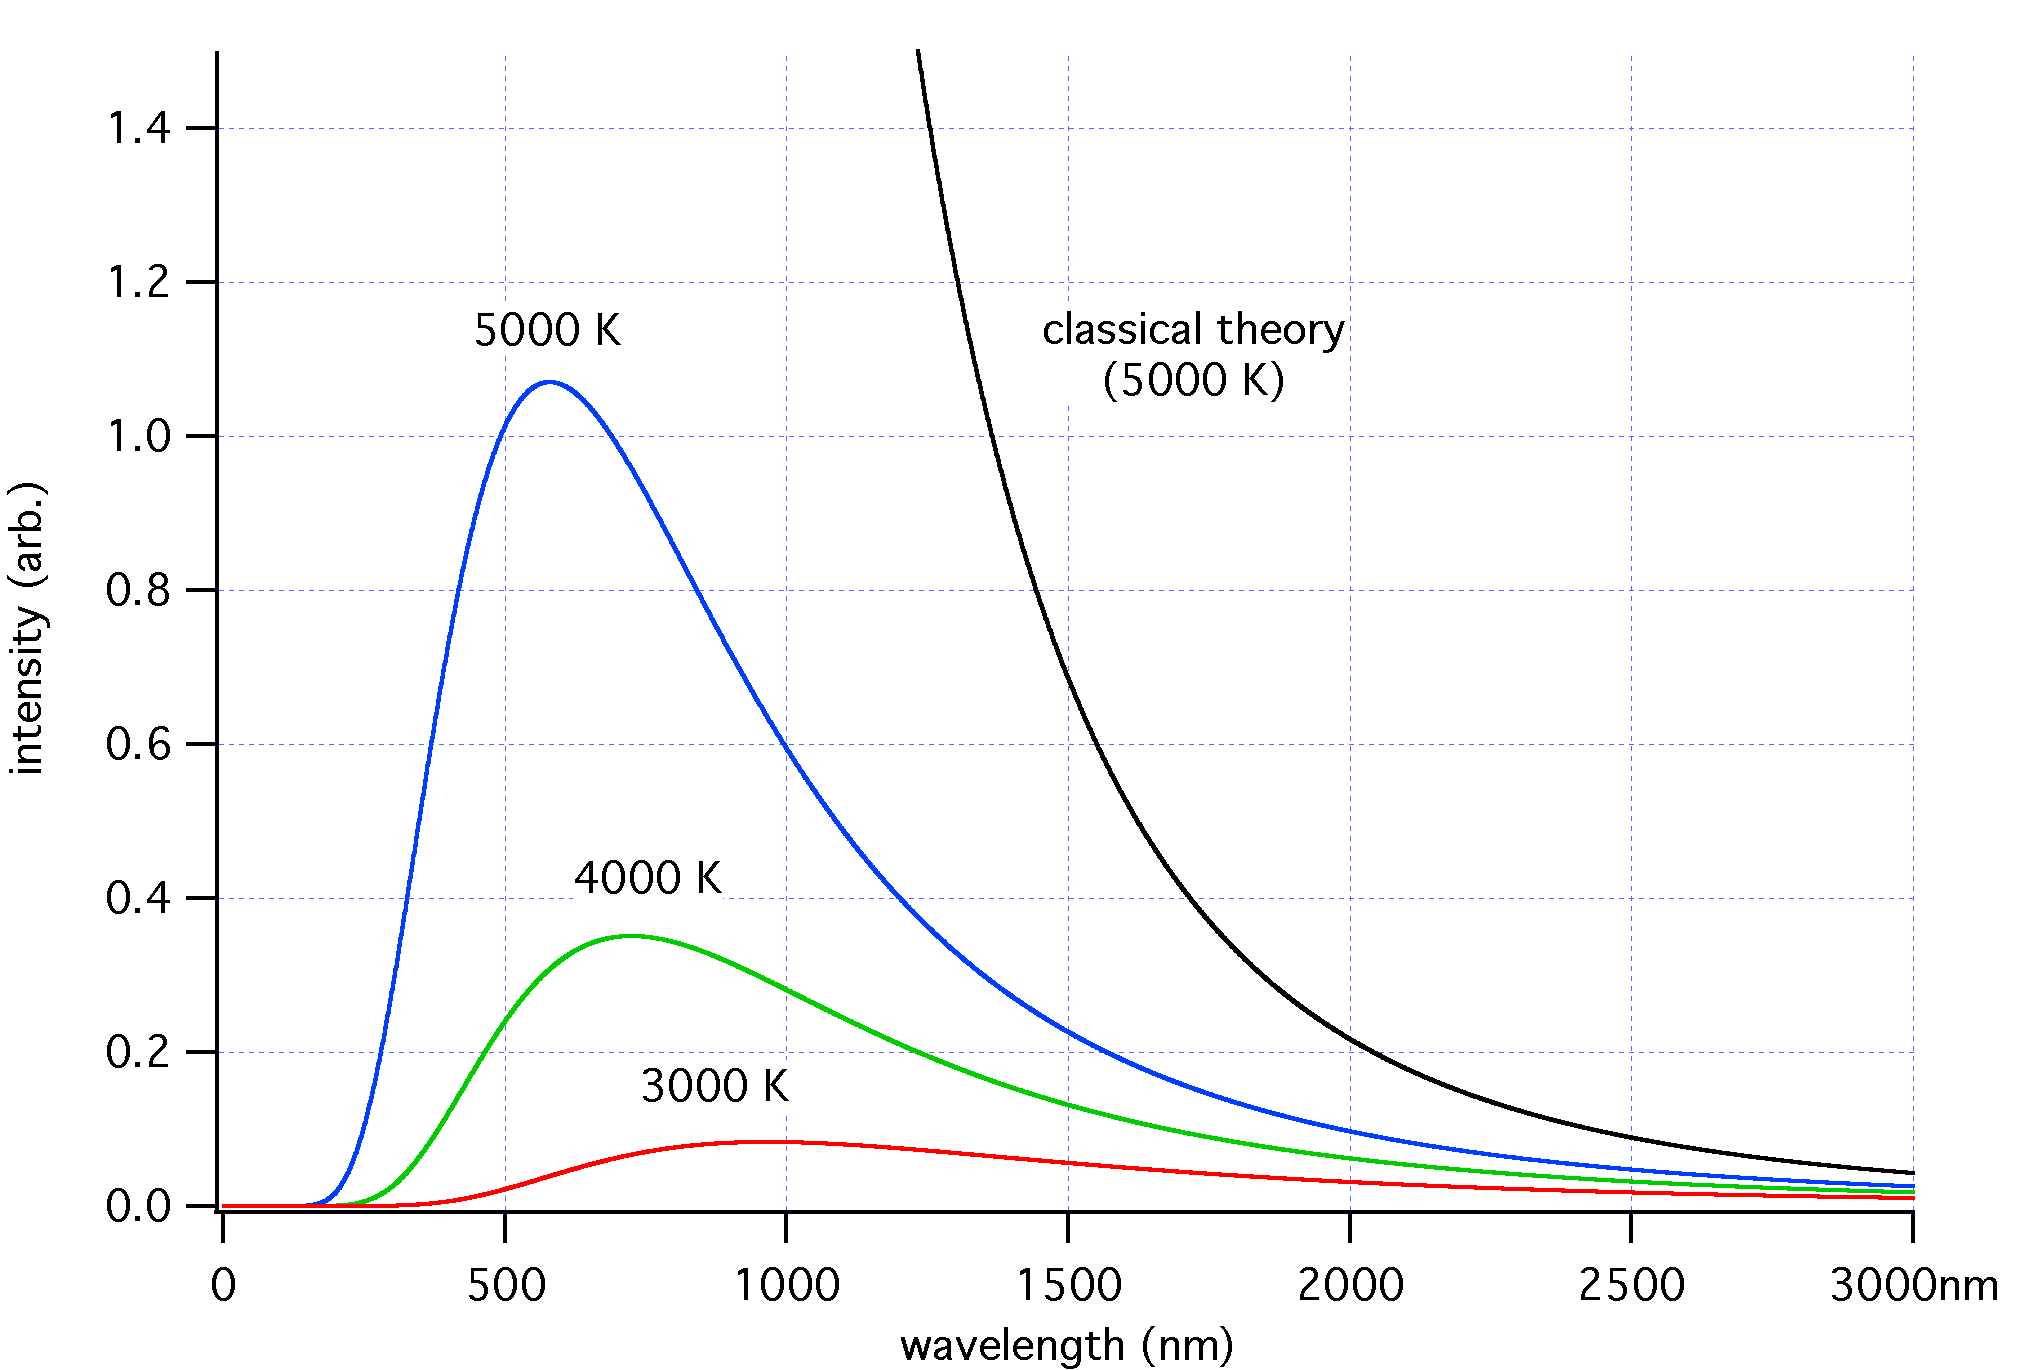
\includegraphics[width=0.5\textwidth]{Pictures/blackbody.png}
  \end{center}
  \caption{Spectre électromagnétique d'un corps chauffé}
\end{wrapfigure}
Tout corps chauffé émet un rayonnement électromagnétique. Un corps noir désigne un objet idéal dont le spectre électromagnétique ne dépend que de sa température. Cette théorie du rayonnement prévoit que le rayonnement émis par un corps chauffé est proportionnel à la température absolue et inversement proportionnel au carré de la longueur d'onde. Cette théorie fonctionne bien pour les longues longueurs d'onde, mais pas pour les courtes, leur spectres est inexplicable par la physique classique. 

En 1900, M. Planck expose ses déductions faites sur ce problème et propose alors l'hypothèse des quanta:  l'énergie n'est pas émise de manière continue, mais par paquets de valeur $$E=h\nu\qquad\text{avec } h = \SI{6.626e-34}{\joule\second}$$
\subsection{Effet photoélectrique}
L'effet photoélectrique est l'émission d'électrons depuis un métal lorsque celui-ci est exposé à des rayons ultraviolets. Les observations sont les suivantes:
\begin{enumerate}
  \item Aucun électron n'est émis en dessous d'une certaine fréquence de rayonnement, valeur caractéristique du métal utilisé.
  \item Les électrons sont émis immédiatement, indépendament de l'intensité lumineuse.
  \item L'énergie cinétique des électrons émis augmente linéairement avec la fréquence du rayonnement. 
\end{enumerate}
En 1905 Albert Einstein trouva une explication à toutes ces observations. Il proposa l'hypothèse que le rayonnement électromagnétique était constitué de paquets d'énergie, les photons.$$E=h\nu=h\frac{c}{\lambda}$$
Si l'on considère le rayonnement électromagnétique comme un rayon de photons, alors l'énergie nécessaire pour retirer un électron d'un métal est symbolisée par la lettre grecque $\Phi$. Si l'énergie du photon est plus grande que $\Phi$, alors l'électron sera émis avec une énergie cinétique définie par la formule: $$E_{\text{cin}}=h\nu-\Phi$$
\subsection{Émission - absorption de photons}
Selon le modèle de Rutherford, un atome émet constamment des ondes électromagnétiques. Ce rayonnement est causé par la ``chute'' des électrons vers le noyau. \newline
Nous avons vu avec le spectre de l'hydrogène que cela n'est vraiment possible. L'existence des photons et la relation entre leur énergie et la fréquence permettent de résoudre ce problème. Nous avons considéré qu'une raie spectrale provenait d'une transition entre deux niveaux d'énergie. Si cette différence d'énergie est emportée par un photon, la fréquence d'une raie d'un spectre est reliée à la différence d'énergie entre deux niveaux d'énergie impliqués dans la transition: $$h\nu=E_{\text{haut}}-E_{\text{bas}}=\Delta E$$
Dans le modèle atomique de Bohr la formule devient beaucoup plus précise grâce à la découverte de plusieurs quantifications visant à éclaircir la disposition des électrons dans un atome.\newline Nous avons en premier lieu la quantification du moment angulaire (avec $\hbar$ la constante de Dirac): $$m\nu r = n\frac{h}{2\pi} = n\hbar$$
Ensuite la quantification des orbites circulaires: $$r_n = \frac{4\pi\epsilon_0\hbar^2}{m_ee^2}n^2$$
Et pour finir la quantification des niveaux énergétiques: $$E_n = -\frac{1}{(4\pi\epsilon_0)^2}\frac{m_ee^4}{2n^2\hbar^2}$$
Avec toutes ces données, il est maintenant possible de calculer la différence d'énergie entre deux couches d'électrons: $$\Delta E = h\nu = \frac{hc}{\lambda} = R_y\left(\frac{1}{n_f^2}-\frac{1}{n_i^2}\right)$$
Avec $R_y$ la constante de Rydberg: $R_y = hcR_{\infty} = \pm\SI{13.605}{\electronvolt} = \SI{2.178e-18}{\joule}$. Le signe de la constante de Rydberg a peu d'importance tant que l'on tient compte de la convention: 
\begin{itemize}
  \item $\Delta E > 0$ si l'atome absorbe (gagne) de l'énergie $(n_i<n_f)$
  \item $\Delta E < 0$ si l'atome émet (perd) de l'énergie $(n_f<n_i)$
\end{itemize}
\begin{figure}[H]
  \centering
  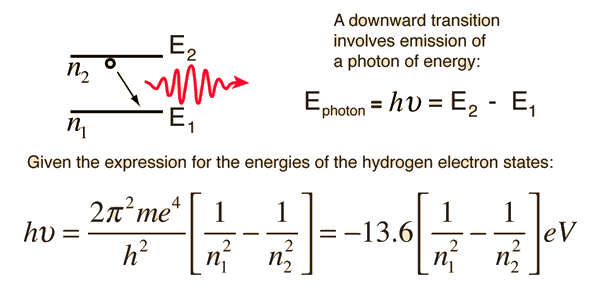
\includegraphics[scale=0.5]{Pictures/hyde}
  \caption{Émission de photons}
  \label{fig:hyde}
\end{figure}
\subsection{La dualité onde-particule de la matière}
L'effet photoélectrique démontre le comportement corpusculaire du rayonnement électromagnétique. Par contre l'observation de la diffraction du rayonnement nous montre qu'il se comporte aussi comme une onde. Cela nous oblige à accepter la dualité onde-particule du rayonnement électromagnétique.\newline
L'hypothèse de De Broglie est l'affirmation que toute matière est dotée d'une onde associé. Selon lui la longueur d'onde et la quantité de mouvement d'une particule sont reliées par l'équation: $$\lambda=\frac{h}{|\vec{p}|} = \frac{h}{m|\vec{v}|} = \frac{hc}{E}\qquad\text{avec }E=h\nu=\hbar\omega$$
\begin{table}[H]
  \centering
  \begin{tabular}{|l|c|c|c|}\hline
    Être humain & $m=\SI{80}{\kilo\gram}$ & $v=\SI{5}{\kilo\meter\per\hour}$ & $\lambda = \SI{6.8e-36}{\meter}$\\\hline
    Grain de sable & $m=\SI{10}{\micro\gram}$ & $v=\SI{1}{\centi\meter\per\second}$ & $\lambda=\SI{6.6e-24}{\meter}$\\\hline
    Électron & $m=\SI{9.1e-31}{\kilo\gram}$ & $E_{\text{cin}} = \SI{1}{\electronvolt}$ & $\lambda = \SI{1}{\nano\meter}$\\\hline
  \end{tabular}
  \caption{Longueur d'onde de De Broglie}
  \label{tab:broglie}
\end{table}
\noindent Avec les formules de De Broglie, on peut facilement retrouver les orbites de Bohr:
\begin{equation*}
  \begin{cases}
    n\lambda &= 2\pi r\\
    \lambda &= \frac{h}{mv}
  \end{cases} \Rightarrow mvr = n\frac{h}{2\pi}
\end{equation*}
\subsection{Fonction d'onde}
Comme les particules ont des propriétés ondulatiore, nous ne pouvons pas nous attendre à ce qu'elles se comportent comme des objets ponctuels se déplaçant sur des trajectoires précises. C'est pourqoi nous associons une fonction d'onde, inventée par Schrödinger, aux particules quantiques: $$\Psi(x,y,z,t)$$
Une fonction d'onde est une fonction mathématique contenant toute l'information sur la dynamique de la particule: position, vitesse, quantité de mouvement, moment angulaire, énergie, \dots\newline
Selon l'interprétation de Born, la probabilité de présence de la particule dans une région est proportionnelle à la valeur de $\Psi^2$ dans cette région.
\begin{align*}
  |\Psi|^2=\Psi\cdot\Psi \qquad& \text{Fonction de distribution de probabilité}\\
  |\Psi|^2dV \qquad& \text{Probabilité de trouver une particule dans un volume $dV$}
\end{align*}
\section{L'atome d'hydrogène}
\subsection{Le principe de nombre quantique}
Afin de trouver les fonctions d'onde d'un électron d'un atome d'hydrogène, nous devons résoudre l'équation de Schrödinger adéquate. Pour cela nous allons utiliser le potentiel coulombien d'un électron de charge $-e$ à une distance $r$ du noyau de charge $+e$: $$U(r) = -\frac{1}{4\pi\epsilon_0}\frac{e^2}{r}$$
Résoudre l'équation de Schrödinger de la forme $$\Psi(r,\theta,\phi,t) = R(r)\Theta(\theta)\Phi(\phi)e^{-iEt/\hbar}$$
\begin{figure}[H]
  \centering
  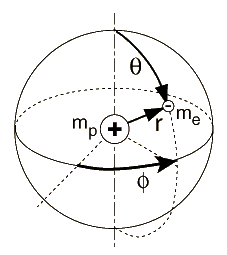
\includegraphics[scale=0.5]{Pictures/schrodinger}
  %\caption{Fonction d'onde}
  \label{fig:schrodinger}
\end{figure}
Schrödinger parvint à résoudre l'équation en définissant les trois fonctions interne à la fonction d'onde: 
\begin{equation*}
  R(r)\propto N_l(r)e^{-\frac{r}{na_0}}; \qquad \Theta(\theta)\propto P_{l,m_l}(\cos{\theta}); \qquad \Phi(\phi)\propto e^{im_l\phi}
\end{equation*}
Dans cet nouvelle équation, nous avons le rayon de Bohr $a_0=\frac{4\pi\epsilon_0\hbar^2}{m_ee^2}=\SI{5.29e-11}{\meter}$, ainsi que 3 nombres quantiques:
\begin{description}
  \item[Nombre quantique principal]: $n=1,2,3,4,\dots$\newline définit l'énergie de l'électron et sa couche électronique.
  \item[Nombre quantique secondaire ou azimutal] : $l=0,1,2,\dots,n-1$\newline définit des sous-couches électroniques.
  \item[Nombre quantique magnétique] : $m_l=0,\pm1,\pm2,\dots,\pm l$\newline définit l'orientation de l'orbitale atomique.
\end{description}
Selon l'équation de Schrödinger, le spectre d'énergie dépend uniquement du nombre quantique principal. Son équation est donc identique aux prédictions de Bohr: $$E_n = -\frac{1}{(4\pi\epsilon_0)^2}\frac{m_ee^4}{2n^2\hbar^2} = \frac{13.60}{n^2}\:\si{\electronvolt}$$
\subsection{Orbitales atomiques}
\begin{wrapfigure}{l}{0.5\textwidth}
  \begin{center}
    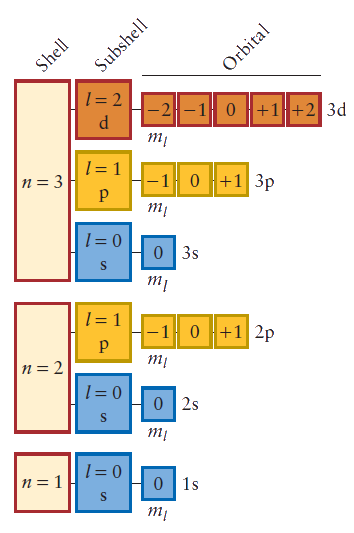
\includegraphics[width=0.48\textwidth]{Pictures/orbitals}
  \end{center}
  \caption{Hiérarchie des orbites}
\end{wrapfigure}
Nous connaisions déjà le nombre quantique principal $n$ qui définit l'énergie de l'orbitale. Les orbitales ayant la même énergie se trouvent sur la même couche de l'atome. À chaque $n$ correspond une couche $K,L,M,N,\dots$ Nous avons ensuite $n$ nombres quantiques secondaires ou azimutals $l$. Ce nombre définit la sous-couche de l'orbitale. À chaque $l$ correspond donc une sous-couche $s,p,d,f,g,\dots$. Pour finir nous avons le nombre quantique magnétique $m$, qui différencie les électrons sur une même sous-couche à l'aide de leur orientation dans l'espace. 

Imaginons que nous souhaitons connaître la probabilité de présence totale de l'électron à une distance $r$ du noyau quelque soit la direction. Nous utiliserons pour cela la valeur de $\Psi^2$ décrit précédemment. La formule que nous cherchons est la fonction de probabilité radiale $$P(r)dr=|\Psi|^2dV=|\Psi|^24\pi r^2dr$$
\paragraph{Représentation}
Les chimistes dessinent habituellement la surface limite d'une orbitale pour la représenter. La forme de cette surface limite dépend de la fonction d'onde. Nous illustrerons deux exemples dans cette synthèse: l'orbitale 2p et l'orbitale 3d.\newline
Il y a trois orbitales p dans chaque sous-couche, correspondant aux nombres quantiques $m_l=+1,0,-1$. Les chimistes ont pris l'habitude de nommer les orbitales selond les axes de leurs lobes.\newline
Une sous-couche $l=2$ est constituée de cinq orbitales. La surface limite d'une orbitale d est plus compliquée que celle d'une orbitale s ou p. Quatre orbitales ont quatre lobes, une est légèrement différente.
\begin{figure}[H]
  \centering
  \begin{subfigure}[b]{0.48\textwidth}\centering
    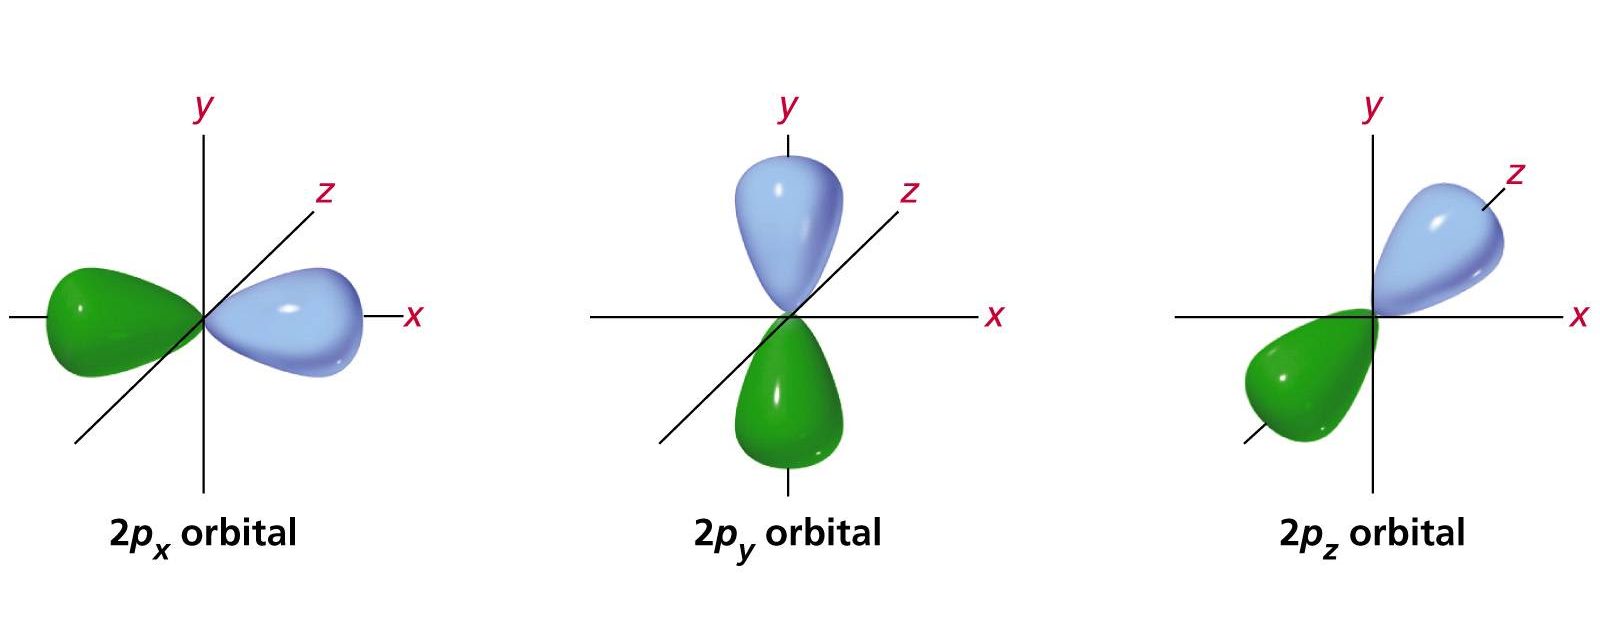
\includegraphics[width=1\textwidth]{Pictures/2p}
    \caption{Orbitales 2p : $m_l=-1,0,1$}
  \end{subfigure}
  \begin{subfigure}[b]{0.48\textwidth}\centering
    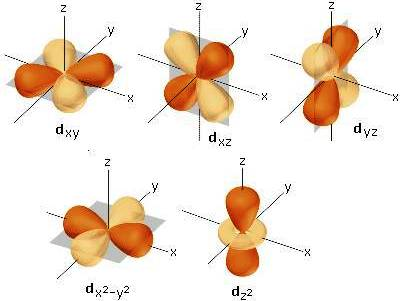
\includegraphics[width=1\textwidth]{Pictures/3d}
    \caption{Orbitales 3d : $m_l=-2,-1,0,1,2$}
  \end{subfigure}
  \label{fig:orbitals}
\end{figure}
\subsection{Spin de l'électron}
L'existence du spin de l'électron a été mise en évidence par l'expérience menée par Stern et Gerlach. Elle consiste à faire passer des atomes d'argent dans un champ magnétique non uniforme de direction verticale. Les atomes d'argent dans leur état fondamental ne disposent que d'un électron célibataire, d'un moment cinétique nul et leur moment magnétique orbital est nul également. Le faisceau d'atomes ne devrait classiquement pas subir l'influence du champ magnétique. Cependant, l'expérience montre que le faisceau se sépare en deux. On explique ce phénomène en introduisant le moment cinétique de spin, ou plus simplement spin.  

Selon la mécanique quantique, l'électron a deux états de spin, représentés par les flèches $\uparrow$ et $\downarrow$. Ces deux états sont désignés par un quatrième nombre quantique, le \textbf{nombre quantique de spin} $m_s=\pm\frac{1}{2}$
\subsection{La structure électronique de l'hydrogène}
Nous pouvons maintenant faire un récapitulatif de ce que nous savons de l'atomes d'hydrogène.
\begin{description}
  \item[Les orbitales] de l'atome sont définies par 3 nombres quantiques: $n,l,m_l$. Les fonctions d'onde de ces orbitales sont les solutions de l'équation de Schrödinger. Ces fonctions d'onde au carré $(\Psi^2)$ calculent la densité électronique de l'atome.
  \item[L'énergie] de l'atome ne dépend que de la couche où se trouve son électron (le nombre quantique $n$).
  \item[Les électrons] de l'atome sont caractérisées par 4 nombres quantiques $n,l,m_l,m_s$.
\end{description}
\section{Les atomes polyélectroniques}
\subsection{Énergies des orbitales}
Un atome polyélectroniques dispose de Z électrons et Z protons. Par rapport à un atome d'hydrogène, un atome polyélectronique a un noyau beacoup plus chargé, charge qui attire plus les électrons et abaisse leur énergie. En plus de ça les électrons interagissent entre eux. L'énergie potentielle totale de l'atome dépend donc de chaque interaction entre les atomes. L'équation de Schrödinger fondée sur cette énergie potentielle est donc extremement difficile à résoudre.

La charge nucléaire effective $Z_\text{eff}$ subie par l'électron est toujours inférieure à la charge nucléaire réelle à cause des effets de pénétration et d'écran des électrons.
\begin{equation*}
  Z_\text{eff} = Z-\sigma\qquad\begin{cases}
    Z&: \text{ nombre atomique}\\
    \sigma&: \text{ constante d'écran}\end{cases}
\end{equation*}
\begin{figure}[H]
  \centering
  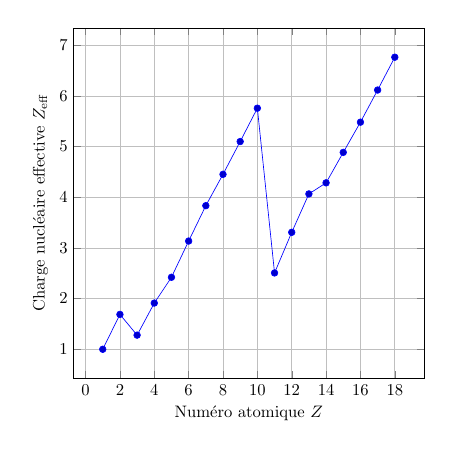
\begin{tikzpicture}[scale=0.6]
    \begin{axis}[
	xlabel={Numéro atomique $Z$},
	ylabel={Charge nucléaire effective $Z_\text{eff}$},
	height=9cm,
	width=9cm,
	grid=major,
      ]
      \addplot coordinates {
        (1,1)
	(2,1.688)
	(3,1.279)
	(4,1.912)
	(5,2.421)
	(6,3.136)
	(7,3.834)
	(8,4.453)
	(9,5.100)
	(10,5.758)
	(11,2.507)
	(12,3.308)
	(13,4.066)
	(14,4.285)
	(15,4.886)
	(16,5.482)
	(17,6.116)
	(18,6.764)
      };
    \end{axis}
  \end{tikzpicture}
  \caption{Charge effective du noyau}
  \label{fig:7}
\end{figure}
\subsection{Effet de pénétration}
La pénétration des électrons décrit la proximité d'un électron d'une orbitale par rapport au noyau. Les électrons bénéficiant d'un plus grand effet de pénétration ont une plus grande charge nucléaire effective. Pour une même valeur $n$, la puissance de pénétration d'un électron suit cette condition: $$s>p>d>f$$
\subsection{Effet d'écran des électrons}
L'effet d'écran fait référence aux électrons de couche plein repoussant les électrons des couches externes. La force d'attraction du noyau sur les électrons des couches externes est donc diminuée par cet effet. L'effet d'écran décrit la quantité de force qu'un électron peut appliqué sur les électrons voisins. Les sous-couches les plus basses ont donc plus d'effet d'écran que les sous-couches supérieurs: $$s>p>d>f$$ 
\subsection{Remplissage des orbitales}
Pour construire la ocnfiguration électronique d'un atome nous allons utiliser le \textbf{principe d'Aufbau}. Ce principe comprend trois règles:
\begin{description}
  \item[Règle de Klechkowsky]: Le remplissage des orbitales se fait par ordre croissant d'énergie.
  \item[Principe d'exclusion de Pauli]: Il ne peut y avoir que maximum deux électrons par orbitale.
  \item[Règle de Hund]: Le nombre d'électrons non-appariés de spins parallèles dans un ensemble d'orbitales de même énergie est maximisé.
\end{description}
À l'aide du diagramme de Klechkowski, on accède à l'ordre de remplissage des sous-couches électroniques d'un élément chimique.
\begin{figure}[H]
  \centering
  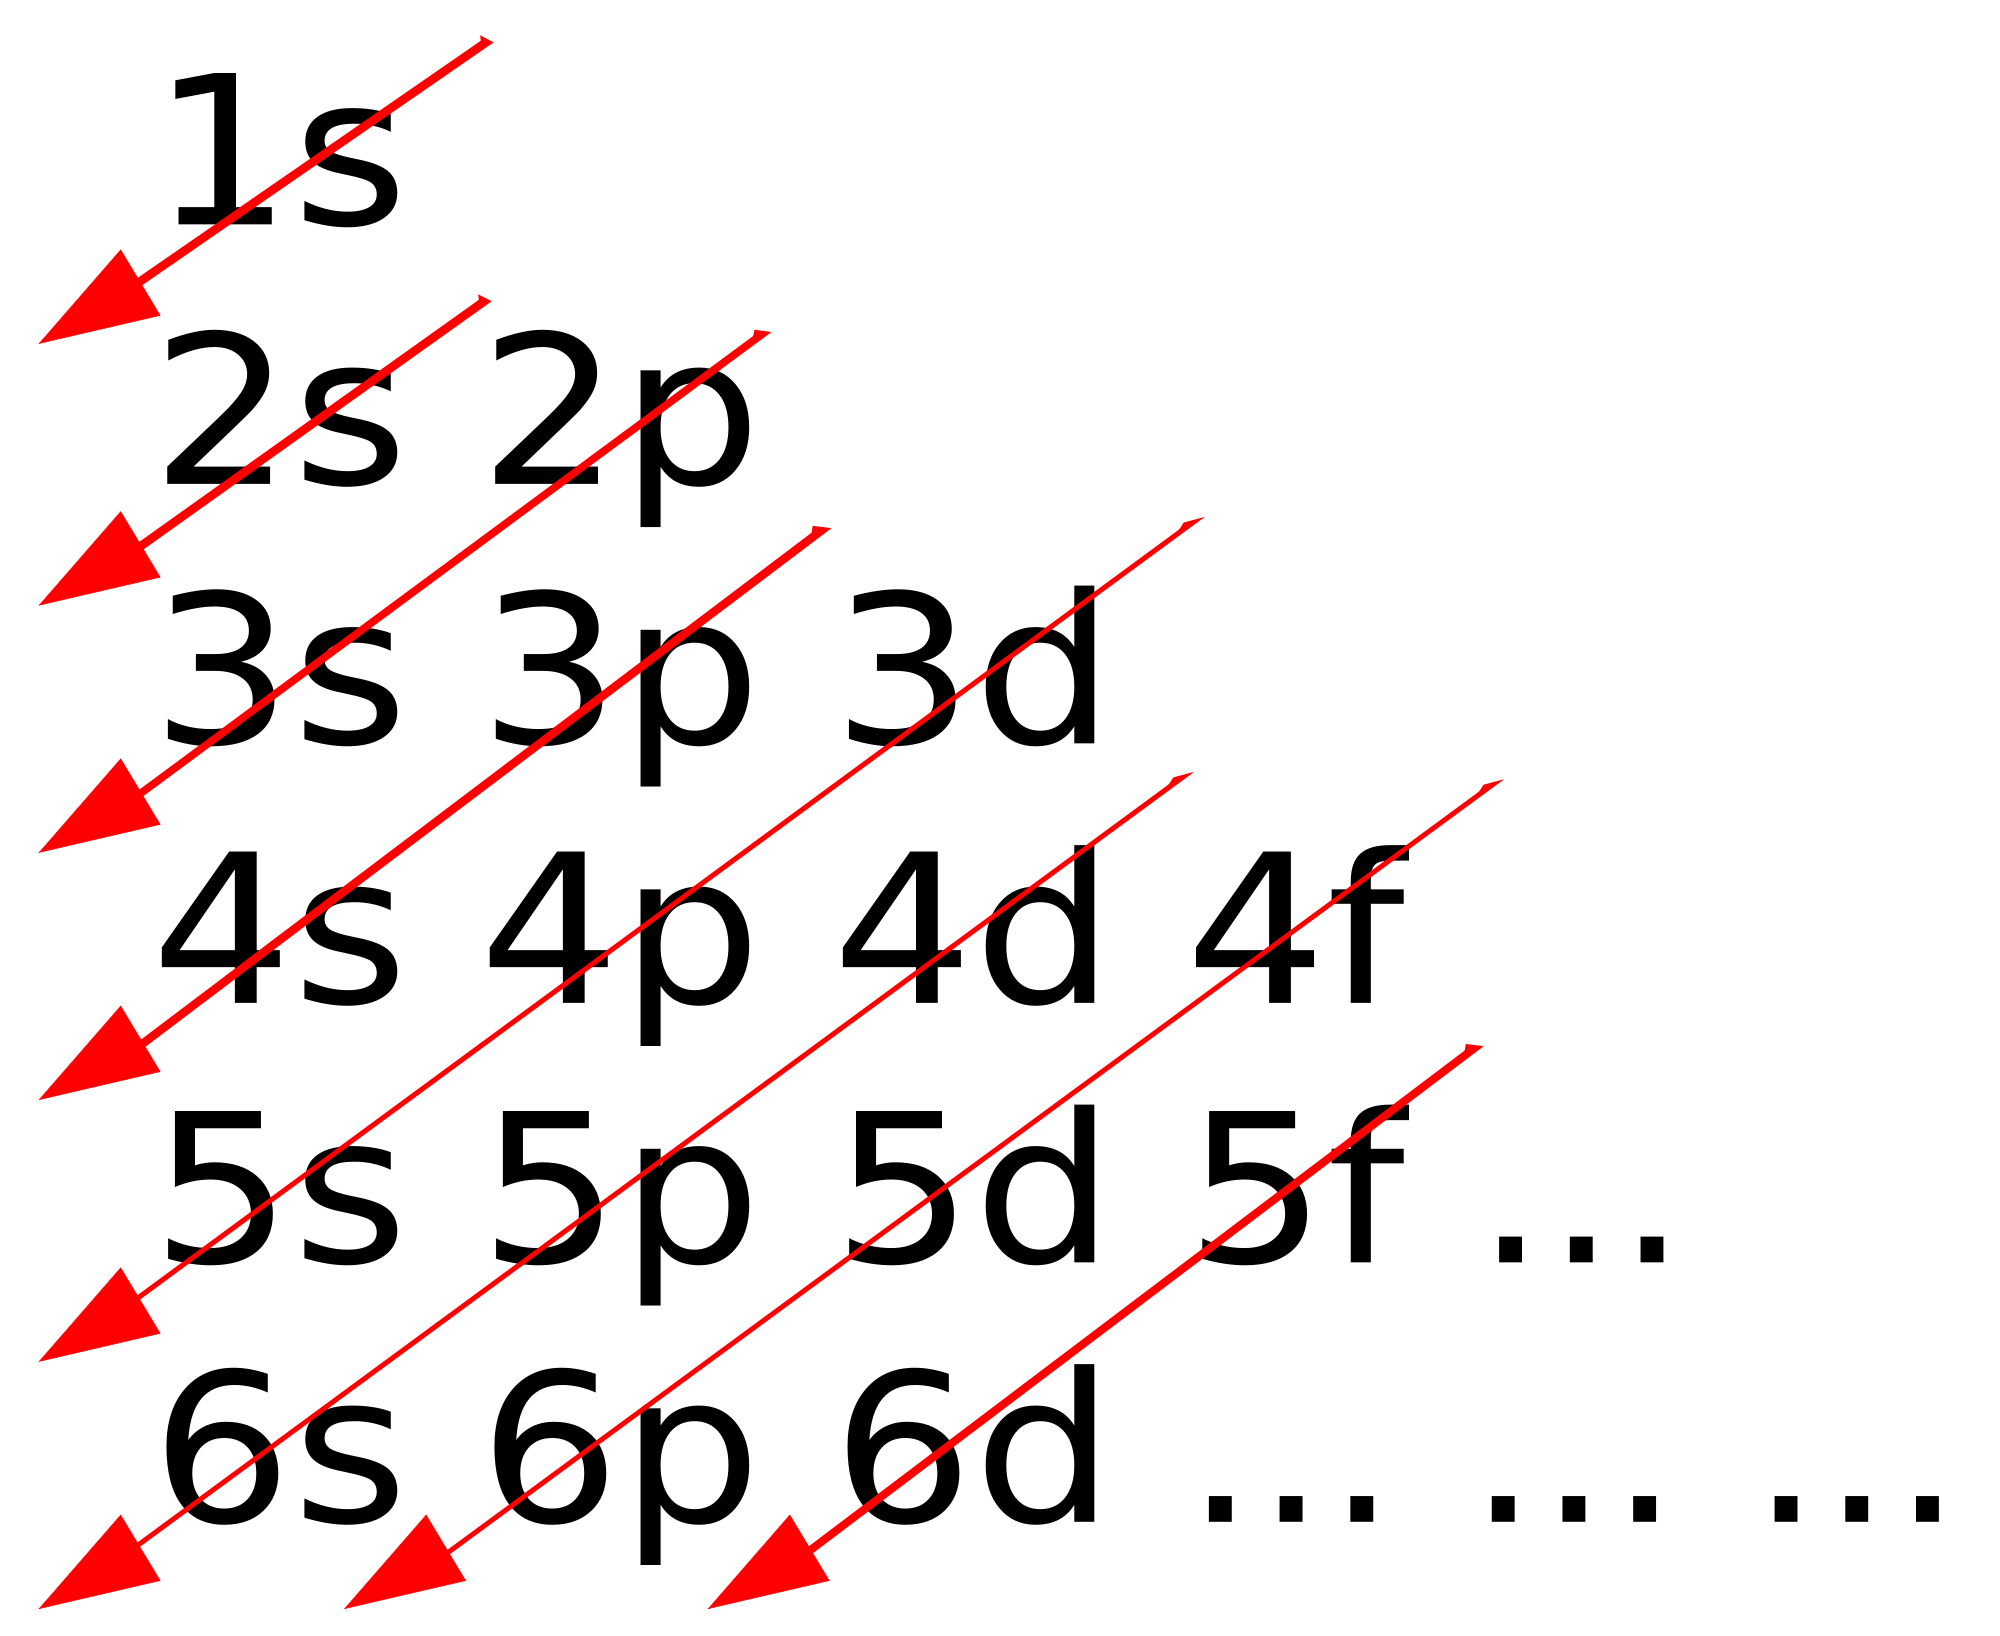
\includegraphics[scale=0.05]{Pictures/diagram}
  \caption{Diagramme de Klechkowski}
  \label{fig:8}
\end{figure}



\end{document}
